\documentclass{book}
\usepackage{mathtools}
\usepackage{tikz}
\usetikzlibrary{positioning}

\usepackage{amsthm}
\usepackage{amsmath}
\usepackage{amssymb}

\newtheorem{defn}[equation]{Definition}
\newtheorem{coro}[equation]{Corollary}
\newtheorem{prop}[equation]{Proposition}
\renewenvironment{proof}{\emph{Proof}}{\qed}


\begin{document}

\tableofcontents


Think about a new outline: 
- Introduce quantities, manifolds, etc. as before. 
- vector as infinitesimal displacement/"line"
- Outer product and K-vectors and infinitesimal K-surfaces
- K-forms as functions of k-vectors
- Integration
- Stokes theorem in diff form
Ch 3
- Symplectic geom (form, ...)
- Riem geom (Inner product, ..)
- ???


\chapter{Mathematical representations of physical objects}


\section{Manifolds and continuous quantities}
\emph{We tell physical objects apart by identifying some measurable properties. In particular, we are interested in properties that are continuous quantities. This gives us manifolds.}

\subsection{Physical objects and quantities}

- \emph{There is a physical object that we want to identify}

Say we're looking at weather. We'll want to know the temperature, wind speed, humidity, whereabouts, etc.

- \emph{We can give real number values describing that object. This gives us quantities}

Fahrenheit, mph, percent humidity, location.
On some set of all possible weather configurations, we look at a specific subset of possibilities described by real numbers. This is our weather report.  

Talking about location on the earth, a \textbf{single space cannot cover the entire earth such that a consistent set of quantities will be defined}. The poles must be in two separate subsets, with separate quantities. 

\begin{defn}
	A \textbf{quantity} is a function $q : U \to \mathbb{R}$ that assigns a measurable value to a physical object.
\end{defn}


- \emph{Having a set of one-to-one quantities sufficient to distinguish one object from another, but not so many that some end up redundant, gives us a coordinate system}


\begin{defn}
	A \textbf{coordinate system} $Q$ is a collection of $n$ quantities $q^i : U \to \mathbb{R}^n$ such that there is a one-to-one relationship between the physical objects in $U$ and elements of $\mathbb{R}^n$.
\end{defn}


\begin{defn}
	A \textbf{coordinate line} is the set of points in $\mathbb{R}^n$ obtained by allowing one quantity to vary and holding the others fixed. 
\end{defn}

\begin{defn}
	A \textbf{coordinate axis} is a coordinate line with the fixed quantities held at 0. 
\end{defn}

- \emph{\textbf{Overlapping} coordinate systems can be transformed between}

Moscow may be seen on both a map of Europe and a map of Asia, so its coordinate system can be swapped. Lisbon, however, will not show up on a map of Asia, so its coordinate system cannot be swapped. 

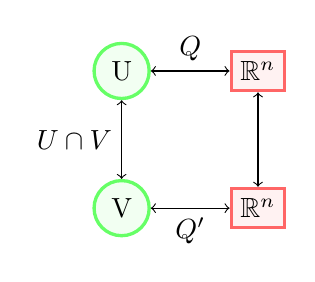
\begin{tikzpicture}
[roundnode/.style={circle, draw=green!60, fill=green!5, very thick, minimum size=7mm},
squarednode/.style={rectangle, draw=red!60, fill=red!5, very thick, minimum size=5mm},
]
\node[roundnode]	(U) {U};
\node[roundnode]	(V) [below=of U]{V};
\node[squarednode]	(realU) [right=of U] {$\mathbb{R}^n$};
\node[squarednode]	(realV) [right=of V] {$\mathbb{R}^n$};

\draw[<->] (U) -- (realU) node[midway, above] {$Q$};
\draw[<->] (U) -- (V) node[midway, left] {$U\cap V$};
\draw[<->] (V) -- (realV) node[midway, below] {$Q'$};
\draw[<->] (realU) -- (realV);
\end{tikzpicture}

\begin{defn}
	Given two coordinate systems  $Q : U \to \mathbb{R}^n$ and $Q' : V \to \mathbb{R}^n$ such that $U \cap V \neq \emptyset$, we call a \textbf{coordinate transformation} the function $f = Q' \circ (Q)^{-1} : \mathbb{R}^n \to \mathbb{R}^n$.
\end{defn}




- \emph{Now that we have sets that can be mapped to the real numbers, we can define manifolds}

For the weather example, a manifold would be all possible weather conditions with a subsection whereon is defined a weather report, measuring temperature, wind speed, etc. in different places. If we're looking to parametrize the entire earth, then our manifold cannot be covered with a single subset, because the earth has poles. We will need multiple subsets to cover all of the earth, and all possible weather conditions. 


 
\begin{defn}
	A \textbf{manifold} is a set of physical objects $X$ such that for any $x \in X$ there exists a $U \subset X$ that contains $x$ and upon which a coordinate system $Q$ is defined.
\end{defn}



\subsection{Sub-manifolds and k-surfaces}

- \emph{Within a manifold can lie a manifold of equal or smaller dimension, with a mapping between them}

If in the original weather report we were worrying about temperature, humidity, and wind speed, we could instead hold one of the three values fixed (say, humidity), and vary the other two. The latter manifold, with humidity held constant, would be a sub-manifold of the former, where all three variables are allowed to change.  



\begin{defn}
	Consider a manifold X of dimension n, and a manifold Y of dimension k, such that $k \leq n$. Y is a \textbf{submanifold} or a k-surface of X if any point on Y is also a point on X. 
\end{defn}

- parameterization of Y can be done in terms of the coordinates of X; $q^i(q'^j)$



\begin{tikzpicture}
[roundnode/.style={circle, draw=green!60, fill=green!5, very thick, minimum size=7mm},
squarednode/.style={rectangle, draw=red!60, fill=red!5, very thick, minimum size=5mm},
]
\node[roundnode]	(X) {X};
\node[roundnode]	(Y) [below=of X]{Y};
\node[squarednode]	(realX) [right=of X] {$\mathbb{R}^n$};
\node[squarednode]	(realY) [right=of Y] {$\mathbb{R}^n$};

\draw[<->] (X) -- (realX) node[midway, above] {$Q$};
\draw[->] (X) -- (Y) node[midway, left] {$U\cap V$};
\draw[<->] (Y) -- (realY) node[midway, below] {$P$};
\draw[->] (realU) -- (realV);
\end{tikzpicture}

What are the possible submanifolds of a given manifold?


\begin{defn}
	For some manifold X of dimension n, $S^k$ is the set of all possible \textbf{k-surfaces}, or sub-manifolds of dimension $k \leq n$, and S $=$ $\cup^n_{k=0}S^k$ is the set of all k-surfaces. 
\end{defn}

A manifold of dimension n can have a boundary of dimension n-1. The boundary itself will not have a boundary.

The boundary of a weather report would be readings restricted to a specific climate. 


\begin{defn}
	Given k-surface $\sigma^k \in S^k$, if for some point $x \in \sigma^k$ you can construct a open neighborhood around x completely within $\sigma^k$, then x is an \textbf{interior point} of $\sigma^k$. 
\end{defn}

\begin{defn}
	Given k-surface $\sigma^k \in S^k$, if some point $x \in \sigma^k$ is not an interior point, then $x$ is a \textbf{boundary point}.
\end{defn}



\begin{defn}
	For k-surface $\sigma^k \in S^k$, the \textbf{boundary operator} $\partial : S^k \to S^{k-1}$ gives the set of boundary points of $\sigma^k$. 
\end{defn}


Dimension is one less since at each section of the boundary, one of the dimensions must be held fixed.

$\partial\partial \sigma^k$ is empty since all points on the boundary are interior with respect to the boundary.


\begin{coro}
	Given $\sigma^k \in S^k$, $\partial \sigma^k \in S^{k-1}$, and $\partial\partial \sigma^k = \emptyset$. 
\end{coro}


NOTE: The boundary appears to be very similar to a line, in that all points on the boundary are interior with respect to the boundary. 

For a cube, the boundary will suffer discontinuities due to the corners. This is ok, since there are a countable number of discontinuities. 

\subsection{Linear Functionals of K-surfaces}

We have the tools now to begin talking about functions along our k-surfaces. 


\begin{defn}
	A \textbf{linear function of k-surfaces}, or \textbf{k-functional}, is a function $f_k : S^k \to \mathbb{R}$ such that for $\sigma^k_1$, $\sigma^k_2 \in S^k$, if $\sigma^k_1 \cap \sigma^k_2 \subseteq \partial \sigma^k_1 \cup \partial \sigma^k_2$, then $f_k(\sigma^k_1\cup \sigma^k_2) = f_k(\sigma^k_1) + f_k(\sigma^k_2)$. 
\end{defn}

\begin{defn}
	$F_k$ is the set of all functionals of dimension k, and $F = \cup_{k=0}^nF_k$ is the set of all k-functionals. 
\end{defn}


\begin{defn}
	$\eth : F_k \to F_{k+1}$ such that $\eth f_k(\sigma^{k+1}) = f_k(\partial \sigma^{k+1})$ is the \textbf{interior operator} on k-functionals. 
\end{defn}

\begin{prop}
	A k-functional applied to the empty set gives zero. 
\end{prop}
\begin{proof}
	
	Let $f_k : S^k \to \mathbb{R}$ be a linear function. Consider the empty set $\emptyset$. 
We have $\emptyset \cap \emptyset \subseteq \partial\emptyset \cup \partial\emptyset$, and $\emptyset = \emptyset\cup\emptyset$. 
So, $f_k(\emptyset) = f_k(\emptyset\cup\emptyset) = f_k(\emptyset) + f_k(\emptyset) \implies f_k(\emptyset) = 2f_k(\emptyset) \implies f_k(\emptyset) = 0$
\end{proof}



\begin{prop}
	Let $f_k \in F_k$ be a k-functional, then $\eth\eth f_k = 0 $.
	
	
\end{prop}
\begin{proof}


	Let $f_k : S^k \to \mathbb{R}$, $g_{k+1} : S^{k+1} \to \mathbb{R},$ and $h_{k+2}: S^{k+2} \to \mathbb{R}$ be linear functions, and let $\sigma^k$ be an element of $S^k$. $f_k(\sigma^k) = g_{k+1}(\partial \sigma^k) = h_{k+2}(\partial\partial \sigma^k) = f_k(\emptyset) = 0$. 
	
	So, $h^{k+2}(s) = 0$ $\forall$ $\sigma^k$, and $h^{k+2}$ is the zero function. 
\end{proof}







\chapter{Mathematical representation of infinitesimal objects}


\section{Differentiable manifolds}

Now that we are able to represent functions along lines as sums of functions along segments, we can start doing calculus. 


- For k-surface $\sigma^k \in S^k$ and k-functional $f_k: S^k \to \mathbb{R}$, $f_k(\sigma^k) = \int_{\sigma^k}f_k(d\sigma^k)$. 

We are interested in studying distribution on manifolds. The limit on infinitesimal areas is a density and requires coordinates to be differentiable.


\begin{defn}
	A \textbf{differentiable manifold} is a manifold $X$ of dimension $n$ such that if there are overlapping subsets $U$ and $V$ with defined coordinate systems $Q: U \to \mathbb{R}^n$ and $Q': V \to \mathbb{R}^n$, then the coordinate transformation $f = Q \circ Q'^{-1}$ is smooth. 
\end{defn}





\section{Vectors and Covectors}

- Starting with the 1D case: for a given line, a vector will be an infinitesimal segment along that line. 


Consider a point P($x^a$).
 
$dP = \frac{\partial P}{\partial x^a} dx^a = \frac{\partial P}{\partial x^b} dx^b = \frac{\partial P}{\partial x^a}\frac{\partial x^a}{\partial x^b} dx^b$

$\implies dx^a = \frac{\partial x^a}{\partial x^b}dx^b $

\emph{Problem with this chain-rule formulation is that the vector isn't the infinitesimal segment}

\emph{Alternative formulation}
$dP = w^ue_u + w^ve_v$

\emph{With this, the infinitesimal segment is the vector, which is what we want in the end. Question remains whether we can still use a chain rule formulation to derive this}

This gives us vectors and covectors: the former being infinitesimal segments, and the latter being functions from vectors to real numbers



\begin{defn}
	A \textbf{vector} is an infinitesimal segment along a line, plane, etc. A \textbf{tangent plane}, then, is a collection of vectors that share a fixed point. 
\end{defn}

NOTE: dx is an element of the tangent space such that if you take dx at all points and sum it, you get the original

\begin{defn}
	A \textbf{differential} $dx$ is the element of the tangent plane such that $x = \int dx$. 
\end{defn}

We can define functions that convert infinitesimal segments to a scalar value. 

For some line P, $\int df(P)$ = $\int \frac{\partial f(P)}{{\partial x^i}} dx^i$ = $\int \frac{\partial f}{\partial x^i}\frac{\partial x^i}{\partial P}dP$ = $\int \frac{{\partial f}}{{\partial x^i}} e^i (dx^j e_j)$


\begin{prop}
	Every linear functional has a corresponding covector, such that for $f : S \to \mathbb{R}$, $f = \int_{\sigma} f(d\sigma)$. In words, a linear functional applied over a line is the same as an integral of a covector over the infinitesimal segments of that line. Further, for $g : S^{2} \to \mathbb{R}$, $g(\sigma) = \int_{\sigma} g(d\sigma) = f(\partial\sigma) = \int_{\partial\sigma}f(d\partial\sigma)$. 
\end{prop}





\section{K-vectors and K-forms}

\emph{Note that electrodynamics has been reworked in the language of k-vectors. Probably a good example to use}




\subsection{K-vectors}

- We want to be able to give a line, surface, body, etc. an orientation. This gives us k-vectors.

- Further, we're now talking about vectors and covectors in arbitrary dimensions

- Here we will be talking about wedge products, and how they behave with k-vectors of different degrees. 



\begin{defn}
	A \textbf{k-vector} is a geometrical object with a dimensionally appropriate magnitude and a direction. A vector as discussed previously is a 1-vector. 
\end{defn}

- \emph{Talking about orientation in terms of quantities: if we flip a quantity, we flip the orientation. Also, it should follow naturally that adding k-vectors of equal magnitude and opposite orientation will give zero.}

\begin{defn}
	$\Sigma^k$ is the set of all vectors of dimension k and $\Sigma = \cup_{k=0}^n \Sigma^k$ is the set of all k-vectors. 
	\end{defn}


\begin{defn}
	
	The \textbf{wedge product} $\wedge : \Sigma^k\times \Sigma^j \to \Sigma^{k+j}$ combines k-vectors antisymmetrically to generate k-vectors of a higher rank. 
\end{defn}

\begin{defn}
	A \textbf{k-form} $\omega_k : V^k \to \mathbb{R}$ is a skew-symmetric linear functional that converts an infinitesimal segment into a scalar value. A covector as discussed previously is a 1-form. 
\end{defn}

\begin{defn}
	$\Omega_k$ is the set of all forms of dimension k and $\Omega = \cup_{k=0}^n\Omega_k$ is the set of all forms. 
\end{defn}






\section{Stoke's Theorem}


\begin{defn}
	\textbf{Stoke's Theorem}: For k-form $\omega_k$ and k-surface $\sigma^k$, $\int_{\partial \sigma^k}\omega_k = \int_{\sigma^k}\Delta\omega_k$. 
\end{defn}

\section{Tensors and coordinate transformations}
Some quantities can undergo one-to-one transformations between coordinate systems. In general, such quantities are tensors. 


\begin{defn}
	A \textbf{tensor} is an object with a one-to-one relationship with objects between coordinate systems. 
\end{defn}

\begin{coro}
	A contravariant tensor of \textbf{rank 1} is a vector, which transforms as  $X'^a = \frac{\partial x'^a}{\partial x^b} X^b$.  
\end{coro}

\begin{coro}
	A covariant tensor of \textbf{rank 1} is a vector, which transforms as $X'_a = \frac{\partial x^b}{\partial x'^a} X_b$. 
\end{coro}

\begin{coro}
	A contravariant tensor of \textbf{rank 2} is a matrix $X^{ab}$ that transforms as $X'^{ab} = \frac{\partial x'^a}{\partial x^c} \frac{\partial x'^b}{\partial x^d} X^{cd}$. 
\end{coro}

\begin{coro}
	A contravariant tensor of \textbf{rank 0} is a quantity $X$ that transforms $X' = X$. Hence, a scalar. 
\end{coro}

- In general, objects associated with covariant tensors will have a lower index, and those associated with contravariant tensors will have an upper index. 












\chapter{Geometry and (States, Tensors, Forms)???}


\section{Symplectic geometry and state spaces}
We want to be able to represent our state configurations. Symplectic geometry arises when trying to describe their areas

\subsection{Symplectic form and areas}



\subsection{Metric tensor}
A more generalized inner product: feed in two vectors, and the outcome is a scalar representing the lengths of the vectors and the angle between them. 

\begin{defn}
	A \textbf{metric tensor g} is a function that takes two vectors and returns a real scalar. 
\end{defn}


\section{Riemannian geometry}
In order to give a mathematically rigorous definition of lengths of vectors and the angle between them, we use an inner product. Vector spaces with an inner product are Riemannian.

\begin{defn}
	Given two vectors $X^a,Y^a \in V$ and a metric tensor $g_{ab}$, the \textbf{inner product} $<X^a,Y^a> : V \times V \to \mathbb{R}$ is defined as $<X^a,Y^a> = g_{ab}X^aY^b$. 
\end{defn}

\begin{coro}
	The magnitude of $<u,v>$ is $|u||v|cos(\theta)$, where $\theta$ is the angle between u and v. 
\end{coro}

\begin{defn}
	If a vector space V contains an inner product, then V is \textbf{Riemannian}.
	\end{defn}



\subsection{Orthogonal basis}

\begin{defn}
	For contravariant vectors $X^a$ and $Y^a$, the two vectors are \textbf{orthogonal} if $<X^a,Y^b> = 0$. 
\end{defn}







\end{document}